\documentclass[11pt,a4paper,oldfontcommands]{memoir}

\usepackage[T1]{fontenc}
\usepackage[utf8]{inputenc}
\usepackage{lmodern}
\usepackage{microtype}
\usepackage[dvips]{graphicx}
\usepackage{xcolor}
\usepackage{times}
\usepackage{csquotes}
\usepackage{mathtools}
\usepackage[
breaklinks=true,colorlinks=true,
%linkcolor=blue,urlcolor=blue,citecolor=blue,% PDF VIEW
linkcolor=black,urlcolor=black,citecolor=black,% PRINT
bookmarks=true,bookmarksopenlevel=2]{hyperref}

\usepackage{geometry}
% PDF VIEW
% \geometry{total={210mm,297mm},
% left=25mm,right=25mm,%
% bindingoffset=0mm, top=25mm,bottom=25mm}
% PRINT
\geometry{total={210mm,297mm},
left=20mm,right=35mm,
bindingoffset=0mm, top=25mm,bottom=25mm}

\usepackage[textsize=tiny,textwidth=3cm]{todonotes}
\setlength{\marginparwidth}{3cm}

\linespread{1.5}

%%% CHAPTER'S STYLE
%\chapterstyle{bianchi}
%\chapterstyle{ger}
\chapterstyle{madsen}
%\chapterstyle{ell}
%%% STYLE OF SECTIONS, SUBSECTIONS, AND SUBSUBSECTIONS
\setsecheadstyle{\Large\bfseries\sffamily\raggedright}
\setsubsecheadstyle{\large\bfseries\sffamily\raggedright}
\setsubsubsecheadstyle{\bfseries\sffamily\raggedright}


%%% STYLE OF PAGES NUMBERING
\pagestyle{companion}\nouppercaseheads 
%\pagestyle{headings}
%\pagestyle{Ruled}
%\pagestyle{plain}
\makepagestyle{plain}
\makeevenfoot{plain}{\thepage}{}{}
\makeoddfoot{plain}{}{}{\thepage}
\makeevenhead{plain}{}{}{}
\makeoddhead{plain}{}{}{}


\maxsecnumdepth{subsection} % chapters, sections, and subsections are numbered
\maxtocdepth{subsection} % chapters, sections, and subsections are in the Table of Contents
\usepackage[french]{babel}
\begin{document}
\title{Développements instrumentaux et simulations Monte Carlo pour la détection des rayons gamma prompts pour le contrôle de l’hadronthérapie}
\author{Simon Martin}
\date{Juin 2020}



\maketitle
\newpage
\tableofcontents
\openany
\chapter{Introduction}
Les cancers sont aujourd'hui une des principales cause de mortalité en France et leur traitement est un des sujets de recherche majeur dans le panorama scientifique actuel. Parmi ces traitements les techniques utilisant des rayonnements ionisants sont utilisé dans prés de 50\% des cas. L'hadronthérapie fait partie de ces traitements, bien que sa part soit encore faible comparée aux techniques utilisant des photons. En utilisant des ion, cette technique permet d'atteindre une grande précision sur la dose déposée. Cependant cette précision est a double tranchant, en cas de mauvais positionnement du patient ou de changements anatomique le faisceau pourrait ne pas traiter la tumeur ou toucher un organe à risque. C'est pour résoudre ce problème que des solutions de contrôle en temps réel de la portée du faisceau d'ions sont investiguées. Une de ces solutions serait de détecté certains photons émis pendant la diffusion d'ions dans le patient appelé gamma prompt (PG en anglais). C'est dans cette optique que des détecteurs spécifique a cette utilisation sont en cours de développement. Des simulations capables de reproduire au mieux l'émission de PG de façon optimale sont développées en parallèle afin de désigner et caractériser ces détecteurs. Nous introduirons ici dans un premier temps l'hadronthérapie pour ensuite se concentrer sur la caractérisation de détecteur BGO servant dans un prototype de caméra PG et enfin nous présenterons le travail effectué sur le module de simulation \enquote{vpgTLE} pour y implémenter la donnée \enquote{Temps de Vol}. 
\openany
\section{Hadronthérapie}
L'hadronthérapie est une technique de traitement utilisant des faisceaux de protons et d'ions légers (comme les ions hélium, carbone et oxygène) et leurs propriétés physiques pour traiter les cancers avec une grande précision. Le termes \enquote{Hadron} de hadronthérapie vient du fais que les particules utilisée sont toute des particules subissant l'interaction forte mais les particules utilisées aujourd'hui en traitement ainsi qu'en recherche sont des ions en très grande majorité, les neutrons étant peu utilisés et les pions ayant été mis à l'écart à la fin des années 80. Depuis 1946 et l'article pionnier de Robert Wilson dans Radiology\cite{wilson} sur l'intérêt thérapeutique des protons, le nombre de centres de protonthérapie a connu une croissance exponentielle. Bien que cette technique soit au stade de l'industrialisation aujourd'hui, des améliorations sont possibles autant sur le plan physique et biologique que technique. 
\subsection{Intérêts}
L'intérêt principal des ions réside dans la forme de la répartition de la dose dans le patient, ils cèdent une grande partie de leur énergie dans les derniers millimètres de leur parcours formant ainsi ce que l'on appelle le pic de Bragg, contrairement à un faisceau de photons qui lui va céder son énergie de manière moins localisé. C'est ce pic de Bragg qui va permettre aux ions de déposer la dose plus localement et d'être plus précis que les photons, épargnant ainsi les tissus sains proches de la tumeur comme le montre la figure \ref{CvsG}. La profondeur de ce pic peut être réglée via l'énergie des ions envoyés, la position du faisceau, elle, sera modifiable soit par un système passif soit par un système actif décrit dans une partie future. La précision de cette technique lui permet d'être utilisée dans des cas où des organes à risque se trouvent proches de la tumeur, notamment pour des cancers oculaires ou spinaux et plus généralement les cancers de la zone ORL. La protonthérapie est également prescrite dans les cas de cancer pédiatrique, les tissus en développement chez l'enfant étant plus radiosensible que ceux de l'adulte, les épargnés devient encore plus une priorité \todo{à reformuler?}\\
\begin{figure}
    \centering
    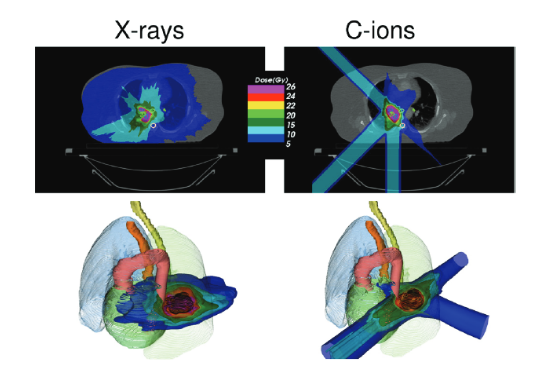
\includegraphics[scale = 0.7]{intro/xrvshDuranteetal2016.png}
    \caption{Comparaison entre un plan de traitement de rayons X et d'ions carbone (Durante et al. 2016) }
    \label{CvsG}
\end{figure}


On définit l'efficacité biologique relative (EBR) comme le ratio entre les doses nécessaires d'hadrons et de photons pour obtenir le même effet biologique.
$$EBR = \frac{D_{hadron}}{D_{photon}}\bigg|_{effet}$$
C'est une quantité complexe qui dépend de beaucoup de facteurs et notamment du poid des paticules. Plus les particules sont lourdes plus la densité d'ionisation dans la cible est élevé, or la densité d'ionisation est directement lié aux dommages causés par les ions. De plus les interactions des photons avec la matière sont aléatoires alors que pour les ions ces interactions se font tout au long de leur parcours. Ils créent donc des zones au niveau du pic de Bragg où la densité d'ionisation est particuliérement élevée, car les interactions sont concentrée et où les réparations de l'ADN seront plus complexes pour la cellule. Ce phénomène est illustré dans la figure \ref{LET} où l'on voit que la concentrations de cassures double brin est importante sur le parcours des ions alors qu'elle est plus disparse pour les photons. Les particules chargées lourdes, tel que les ions, ont un LET élevé ce qui leurs permet d'avoir un effet biologique plus important que des photons pour la même dose et donc d'avoir un EBR supérieur à 1 au niveau du pic de Bragg où la densité d'ionisation est maximale. En clinique l'EBR vaut  pour des protons entre 1.1 et 1.2 et pour des ions carbone entre 2 et 5 \cite{Choi}. 
\begin{figure}
    \centering
    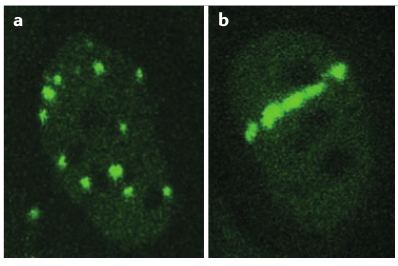
\includegraphics[scale = 0.7]{intro/LETDSS.png}
    \caption{Concentration des cassures doubles brins dans une cellule de culture prélever d'un osteosacrome chez un patient pour (a) une exposition à des rayons X et (b) à des ions carbone. Les cassures double brins sont visualisé grâce à de l'immunofluorescence marquant les histones $ \gamma$ H2AX (Durante et al. 2017)}
    \label{LET}
\end{figure}
\subsection{Défis}
Malgré l'augmentation du nombre de centres et une industrialisation progressive de la technique, l'hadronthérapie reste une technique coûteuse et sa rentabilité est difficile à évaluer \cite{LIEVENS2013134}. Un centre d'hadronthérapie peut coûter entre 3 fois (pour la protonthérapie), et 7 fois (pour la thérapie par ions carbone), plus cher qu'un centre de traitement par rayons X dernière génération \cite{Nupecc}. Des avancées pour rendre les accélérateurs plus compacts et moins chers sont donc encore nécessaires.


La balistique précise des ions n'est pas encore utilisée de façon optimale, la technique étant très sensible aux changement anatomique, aux erreurs de placement ainsi qu'à l'incertitude de la conversion des unitées hounstfield obtenu d'image RX mais utilisé pour des ions\cite{Paganetti2012}. Une marge de sécurité de l'ordre de 2-3mm est donc appliqué au volume cible planifié. Cette marge pourrait être réduite en utilisant des moyens de monitoring direct tel que le monitoring TEP \cite{ENGHARDT2004284} ou Prompt Gamma \cite{PGMonitoringC12}. Nous nous intéresserons plus particulièrement à ce derniers dans la suite de ce rapport. \\
Des simulations visant à être plus rapide que les simulations MC classique tout en restant aussi précise sont en cours de développement \cite{Huisman_2016}\cite{Embriaco_2018}\cite{Sterpin_2015}. Celles ci permettraient d'obtenir un profil gamma prompt attendu pour le comparée à celui mesurée.

\section{Création et délivrance d'un faisceau d'ion}
Les premiers accélérateurs utilisé en hadronthérapie étaient destinés en première intention à la physique nucléaire et à la physique des particules. ils n'étaient donc pas vraiment adapatés aux irradiations médicales. Pour pouvoir traiter des lésions profondes, l'énergie du faisceau d'ions doit être modulable de façon à pouvoir atteindre une profondeur allant jusqu'à 25 cm. Ce faisceau doit également être capable d'être déplacé précisément dans le plan perpendiculaire à sa direction de propagation pour pouvoir impacter tout le volume à traiter. Pour satisfaire ces conditions deux méthodes d'accélération sont utilisées actuellement, le cyclotron, principalement utilisé en protonthérapie, et le synchrotron, utilisé pour les ions.

Un cyclotron est composé de deux électrodes vides. Une tension variant de façon alternative est appliquée entre elles et permet d'accélérer les particules chargées. Un champ magnétique perpendiculaire au plan du cyclotron permet d'obtenir une trajectoire circulaire. Le faisceau ainsi créé possède une intensité fixe et réglable mais avec une énergie fixe. Pour pouvoir faire varier cette énergie, et régler ainsi la profondeur du pic de Bragg, on utilisera un système passif sur la ligne du faisceau. Ce système est composé d'un premier diffuseur qui va élargir le faisceau relativement étroit en un faisceau homogène et large et d'un deuxième diffuseur qui va venir étaler le pic de Bragg. Il va pouvoir ainsi traiter sur toute une gamme de profondeur. Un compensateur situé au niveau de la peau du patient qui va venir limité le faisceau à la forme du volume traité.

Les synchrotrons, eux, utilisent une trajectoire dont le rayon de courbure est maintenu fixe grâce à un champs magnétique qui varie de façon à garder la particule dans leur enceinte jusqu'à ce qu'elle atteigne l'énergie voulue. Contrairement aux cyclotrons, les synchrotrons ont la possibilité de faire varier rapidement l'énergie du faisceau délivré sans système externe mais présente une intensité plus faible. Les synchrotrons sont également beaucoup moins compacts ; ils font une taille de 10~m pour les protons et 30~m pour les ions carbone. Un système actif sera privilégier pour répartir la dose: ce système est composé de deux aimants permettant d'orienter la trajectoire du faisceau dans le plan perpendiculaire à la direction de propagation du faisceau. La profondeur est quant à elle réglée via l'énergie du faisceau. Ce système permet une meilleure conformité du faisceau et n'utilise pas de matériel externe dépendant du patient, ce qui permet de réduire la dose induite par les neutrons. L'inconvénient est que ce type de système de délivrance est plus sensible aux mouvements d'organe. 

\begin{figure}[h!]
    \centering
    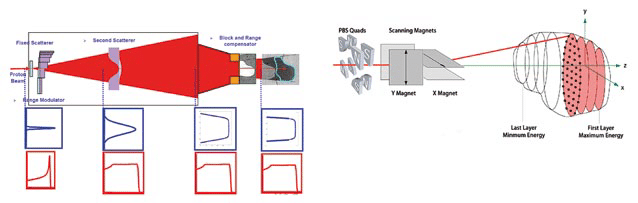
\includegraphics [scale = 0.7]{intro/Passive-left-and-active-right-beam-delivery-system-courtesy-of-IBA.png}
    \caption{Comparaison entre un système de délivrance du faisceau passif (gauche) et actif (droite) (Rapport Nupecc 2014)}
    \label{fig:my_label}
\end{figure}
\openany
\section{Interaction ion-matière}
\subsection{Physique des interactions}

%\todo{Cela n'a pas de sens de parler d'interaction inélastique avec les électrons puisque les électrons sont des particules élémentaires qui ne peuvent avoir d'énergie interne d'excitation. Il faut parler de collisions inélastiques avec les atomiques cibles ou d'interaction avec les électrons.}\todo{Je pense qu'il est plus juste et plus simple de distinguer les interactions avec les électrons (en fait avec les atomes ou molécules) et les interactions avec les noyaux atomiques. Pour éventuellement détailler ensuite les différents types de ces 2 grands types d'interactions.}
Il est possible de séparer les interactions entre les ions et la matière en 2 catégories, la première correspondant aux interactions entre les ions et le nuage électronique des atomes et la seconde aux interactions entre les ions et les noyaux de ces même atomes. L'interaction entre un ions et le nuage électronique est de type électromagnétique (EM) inélastique. La deuxième catégorie regroupe deux interaction, une première EM élastique et une deuxième nucléaire. D'autres interactions sont possibles mais sont négligeables dans le cadre de l'hadronthérapie.\\
\begin{figure}[h!]
    \centering
    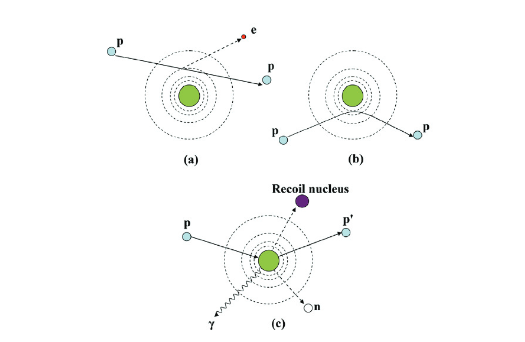
\includegraphics{intro/Newhauser2015.PNG}
    \caption{Schéma des différentes interactions d'un protons dans la matière: EM inélastique (a), EM élastique (b) et nucléaire (c) (Newhauser et. al 2015)}
    \label{fig:my_label}
\end{figure}

Les interactions EM inélastique avec le nuage électronique sont la principale source de perte d'énergie du faisceau d'ions.  Ces interactions sont décrit par la formules de Bethe et Bloch. La dépendance du pouvoir d'arrêt en $1/\beta^2$ (avec $\beta = \frac{v}{c}$) implique que plus la particule est rapide plus le pouvoir d'arrêt est faible et ainsi le pouvoir d'arrêt maximal est atteint à la profondeur du pic de Bragg pour une vitesse égale à $v_p = z^{\frac{2}{3}}v_0$ avec $v_0 = e^2/\hbar$ la vitesse de Planck et $z$ la charge de la particule. 

Bien qu'ayant une part moins importante les interactions coulombienne avec les noyaux de la cible participent également à la distribution de la dose. Elles ont notamment un rôle important dans la diffusion latérale du faisceau.

En plus des interactions EM, les réactions nucléaires participent également au pouvoir d'arrêt bien qu'ayant une part moins importante. Ces interactions peuvent être décrites en deux étapes : une première étape où l'ion entre en collision avec le noyau cible et une deuxième où les noyaux excités par la collision se désexcitent en émettant des particules secondaires. Seulement une partie des nucléons sont impliqués dans le processus de collision (ce nombre de nucléons dépend du paramètre d'impact de la collision b correspondant à la distance entre le point d'impact et le centre du noyau) ces nucléons créent ainsi une zone appelée \enquote{boule de feu} tandis que les nucléons spectateurs formeront des fragment \enquote{projectile ressemblant} et \enquote{cible ressemblant}. Ce sont tout ces fragments qui émettront des particules secondaires durant le deuxième processus, parmi ces particules secondaires des protons, des neutrons et des rayons gamma appelés \enquote{gammas prompts}.\todo{La définition de 3 sources de gammas ici ne me semble pas pertinente : les 511 keV ne sont pas des gammas prompts. Et les gammas générés lors des réactions nucléaires subies par les neutrons secondaires sont aussi des gammas prompts.} %Ces gammas proviennent de trois sources différentes; les prompt gammas issu de la désexcitation direct des noyaux, les gammas issus de l'annihilation de positrons émis par les noyaux et  les gammas issu de l'interaction entre les neutrons émis par les noyaux et la cible. Les deux première sortent de gamma sont utilisé pour le contrôle de l'hadronthérapie tandis que les gammas issu de neutrons participe au bruit de fond.


\openany
\section{Contrôle du parcours des ions lors de l'hadronthérapie}

\subsection{\'Etat de l'art}

Deux techniques majeures sont aujourd'hui étudiées : la première utilise les rayons gamma issus de l'annihilation de positons produits par des noyaux radioactif émmetteur $\beta^+$, qui peuvent eux mêmes être produit par une intéraction avec un ion, et l'autre basé sur la détection de gammas prompts. Nous nous intéressons plus particulièrement à cette dernière mais une description détaillé du contrôle TEP peut être trouvée dans Parodi (2015) \cite{Parodi20157153}. La détection de gammas prompts pour le contrôle de l'hadronthérapie est une technique prometteuse car d'une part le gammas sont émis très rapidement, moins d'une nanoseconde après l’interaction nucléaire entre un ion et sa cible, et d'autre part la corrélation du profil gamma prompts avec celui de la dose a été vérifié par \cite{PGMonitoringC12}pour les ions carbone et par \cite{Min2006} pour les protons. Plusieurs propositions ont été émise pour la détection de ces gammas et plusieurs prototypes existe dans le monde aujourd'hui. Ces prototypes peuvent être séparés en deux catégories, ceux produisant une image et ceux qui n'en produise pas. Dans la première catégorie une collimation est nécessaire pour obtenir une image après reconstruction, elle peut être de deux types, physique, en utilisant un collimateur matériel ou électronique à l'aide d'une caméra Compton. 

\subsubsection{Systèmes ne produisant pas d'image}
Ces systèmes ont pour vocations de comparée des données en temps ou en énergie recueillies pendant le traitement à des données attendue pour en déduire la conformité de la délivrance du traitement. Ces techniques ne nécessitant pas d'information spatiale, les détecteurs utilisés demandent des spécifications moins contraignantes et donc coute moins chère et sont plus facilement intégrable à la salle de traitement.\\
Deux de ces techniques utilisent la donnée temps de vol (\enquote{Time of Flight} ou ToF en anglais). La première \enquote{Prompt Gamma Timing} (PGT) initié par \cite{Golnik_2014} propose d'utiliser le lien qui existe entre temps de vol des gamma prompts et parcours des protons. Des différence de parcours allant jusqu'à 2 mm pour des fantômes hétérogènes définit ont put être détectée \cite{Hueso_Gonz_lez_2015}. La deuxième \enquote{Prompt Gamma Peak Integral} (PGPI) utilise l'intégrale de la distribution ToF des PG pour détecter un surdosage ou un shift dans le parcours des ions, un shift de 3~mm a put être détecté \cite{KrimmerPGPI}. TIARA ???\\
La technique \enquote{Prompt Gamma Spectroscopy} (PGS) propose de déduire le matériel traversé par le faisceau d'ions à partir des raies caractéristique du spectre PG. La section efficace d'interaction variant avec l'énergie des ions incident il est également possible de déduire l'énergie des ions  à partir de la hauteur de ces raies. En étudiant ainsi la composition de la cible \cite{Testa_2014} a réussi a obtenir une précision de 4~mm dans un cas de cancer de la prostate.

\subsubsection{Caméra Collimatée}
La caméra collimatée utilise une collimation physique discriminant les photons arrivant dans le détecteur sur leur endroit d'émission et obtenir ainsi une information spatiale sur le parcours des ions. Un deuxième tri peut être effectué en utilisant la donnée ToF afin de trier les PG issu de neutrons secondaire. La collimation utilisé peut être de deux types, à fentes parallèles ou de type \enquote{knife-edge}.\\
Le collimateur à fentes présente de longues fentes parralléles composé d'un matériau lourd, tel que le tungsten, afin d'absorber les photons n'arrivant pas avvec une incidence normale dans le détecteur. Afin d'optimiser son design des simulations ont été menées \cite{Pinto_2014}\cite{MinSimu}. Des différences de parcours de l'ordre de 1-2~mm ont put être observées dans des cibles hétérogènes \cite{PintoCollimated}.\\
Le collimateur \enquote{knife-edge} utilise le principe optique du même nom. IBA et Poltecnico Milano ont dévellopé \enquote{HiCam} \cite{Smeets_2012} et a été testé en clinique par \cite{Richter2016}, La caméra a ainsi put détecter des variations allant jusqu'à 2~mm. La présence d'un collimateur physique qui absorbe certains photons diminue le nombre de photons détectés et diminue donc l’efficacité de détection, dans la prochaine section nous allons introduire un système ne se servant pas de collimateur physique pour  augmenter cette efficacité.  

\subsubsection{Caméra Compton}
La caméra Compton utilise un principe de collimation électronique basé sur la détection de deux (ou plus) interactions entre un photon et un détecteur stratifié. Une image pourra être ensuite reconstruite à l'aide des cônes de réponses obtenu grâce a la cinématique Compton ainsi qu'aux positions d’interactions et de l'énergie déposée par celles-ci. Cette méthode de détection est bien adapté à la détection de gamma prompts ceux ci étant émis avec une énergie de quelques MeV favorisant l'interaction Compton. Dans sa version la plus simple la caméra Compton se compose de deux éléments, un diffuseur et un absorbeur. Dans cette conformation l'absorption totale du photon dans l'absorbeur est nécessaire, on peut palier à ce problème en ajoutant un diffuseur au prix cependant d'une perte majeure d'efficacité de détection. En utiisant la composition de la cible des algorithme sont capbles de n'utilisé que certaines raies caractéristique du spéctre gamma prompt émis et ainsi reconstruire une image \cite{Draeger_2016}. Des algorithmes de reconstructions analytiques basé sur la transformée de radon conique sont en cours de développement \cite{Maxim_2018}.

\subsection{Projet CLaRyS}

Le projet CLaRyS (Contrôle en ligne de l’hadronthérapie par rayonnements gamma secondaire) est une collaboration entre 4 institutions françaises (IP2I-Lyon, LPSC-Grenoble, CPPM-Marseille, CREATIS-Lyon) se concentrant sur le développement de détecteur gamma pour le contrôle en ligne de l'hadronthérapie. Deux prototypes sont en cours de développement, une caméra compton et un caméra collimatée a fentes parallèles. Ces deux protoypes partagent le même absorbeur constitué de bloc de BGO et le même marquage temporel du faisceau réalisé par un hodoscope toutes ces parties sont reliés via un système d'acquisition décris dans \cite{Caplan_2019}. Les détecteurs de BGO sont issus d'une caméra TEP phillips et sont constitués d'un bloc de BGO $3.5 * 3.8 * 3$~cm$^3$ divisé en $8*8$ pseudopixels relié a 4 photomultiplicateurs. Chaque bloc doit être caractérisé en espaces en énergies et en temps. Un premier travail de caractérisation a été éfféctué par \cite{Fontana_2018} mais des mesures faisceau au Centre Antoine Lacassagne (CAL) de nice ont montré que le faisceau était trop intense ...


\section{Simulations numériques de l'émission des rayons gamma prompts}

\subsection{\'Etat de l'art}

Le contrôle en temps réel des rayons gamma prompts (prompt gamma (PG) en anglais) repose sur la caractérisation, en amont, de la réponse des détecteurs dans différentes situations. Il est égalemnt nécessaire d'avoir une éstimation du signal attendu pour pouvoir le comparé au signal mesuré.  Pour cela différentes techniques de simulation ont été utilisées. Des simulations Monte Carlo classiques ont été menées mais celles-ci demandent un temps de calcul élevé \cite{KRIMMER201858}, notamment à cause de la rareté d'émission des PG. D'autres méthodes ont été développées pour réduire ce temps de calcul \cite{Qin_2017}. Parmi elles, des techniques analytiques \cite{Sterpin_2015} mais aussi des techniques de réduction de variance ont été développées, notamment la technique \enquote{vpgTLE} basée sur une estimation de la longueur de trace dans les voxels de la géométrie simulée (\enquote{vpgTLE} : voxelized prompt gamma Track Length Estimator).

\subsection{La technique \enquote{vpgTLE}}

Une première version \enquote{pgTLE} de cet outil a été développée pour les fantômes définis de manière analytiques \cite{El_Kanawati_2015}. Le gain en temps de calcul de cette version était estimé à $10^5$. Huisman \textit{et. al} ont proposé ensuite une version \enquote{voxélisée} (\enquote{vpgTLE}) fonctionnant pour tous les types de faisceau et de fantômes et accomplissant un gain d'efficacité de $10^3$ \cite{Huisman_2016}. \enquote{vpgTLE} est divisé en 2 parties : dans la première partie, c'est l'interaction des protons avec la cible qui est simulée afin d'obtenir les PG générés dans la cible avec à la fois la position d'émission et l'énergie du gamma  ; dans la deuxième partie de la simulation, les gammas sont propagés dans la géométrie simulée incluant le système de détection. L'énergie des gammas générés est tirée aléatoirement dans une base de données contenant le spectre des PG en fonction de l'énergie des protons incidents pour différents matériaux cible. Cette base de données est pré-calculée une fois pour toutes (avec un ensemble donné de modèles physiques (\enquote{physicslist})).

Le deuxième objectif du stage (en parallèle du travail de caractérisation des blocs BGO) consistait à intégrer dans le module \enquote{pgTLE} l'information temporelle, c'est-à-dire le temps d'émission du PG. Cette information est nécessaire pour toutes les techniques de détection PG utilisant la mesure de temps de vol soit pour réduire le bruit de fond induit principalement par les neutrons secondaires (caméras gamma avec temps de vol, technique PGPI, technique PGS) soit pour obtenir une information indirecte sur le parcours des ions (PGT, TIARA).


\openany
\chapter{Caractérisation de blocs BGO pour la détection de rayons gamma prompts}



\chapter{Modélisation de l'émission des rayons gamma par simulations Monte Carlo hybrides (vpgTLE)}

\section{Introduction}

\todo{Commencer par donner des ordres de grandeurs de la mémoire qui serait requise dans le cas où nous souhaiterions corréler énergie et temps d'émission des PG.} Nous montrerons dans un premier temps qu'il est raisonnable de stocker le temps de vol et l’énergie de façon indépendante, pour cela nous avons étudié trois cas, un cas homogènes simple et cas hétérogènes très défavorables ainsi qu'un cas réaliste. 

\section{Matériel et méthodes}

\subsection{\'Etude de la corrélation entre énergie et temps d'émission des gammas}

Nous présentons ici trois cas, le premier représente un fantôme homogène uniquement constitué de PMMA qui nous servira de comparaison pour le deuxième fantôme décrit par Parodi et. al \cite{1487723} qui représente un cas fortement défavorable et enfin le un dernier cas réaliste tiré d'un plan de traitement et d'une image CT décrit dans Huisman et al. (2016). Nous nous intéresserons à la distribution en énergies temporelles des protons et de leurs PG produits.\\ Pour cela nous utiliserons Gate 8.2 avec la liste physique QGSP BIC HP EMY, nous stockerons dans un premier temps l'énergie des protons ainsi que leur temps de vol pour ensuite tiré 50 énergies différentes dans leur spectre PG associé, issu de la base de données pré-calculé, dans le matériau du voxel d'intérêt.\\
Pour les deux premiers fantômes nous utiliserons un faisceau de protons circulaire gaussien de 150~MeV avec un écart-type de position de 3.5~mm et un écart-type angulaire de 0.002~rad. Pour le dernier fantôme nous utilisons le même que faisceau que précédemment mais réduit à 130~MeV ainsi qu'un faisceau issu d'un plan de traitement avec une couche distal de 133.08~MeV et 7 spots. Tout les faisceaux sont constitué de $10^6$ protons. 

\subsubsection{Fantôme homogène}

Le fantôme utilisé est composé uniquement de PMMA de dimension $221*70*70$~mm$^3$. L'axe du faisceau est décalé de 7 mm en dessous de l'axe de fantôme. On s'intéresse à trois volumes de $0.5*0.5*0.5$~mm$^3$, un premier situé dans l'axe du faisceau avant le pic de Bragg situé à 120.5~mm de profondeur un autre situé à la même profondeur mais excentré du faisceau et un dernier situé dans le pic de Bragg à 130.5~mm de profondeur.\\
\begin{figure}[h!]
    \centering
    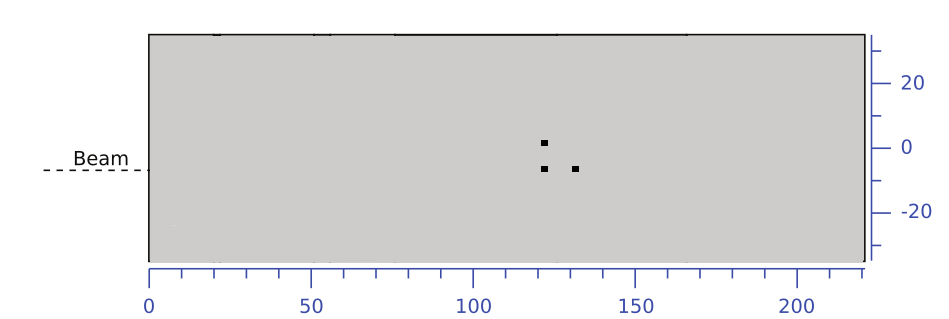
\includegraphics[scale = 0.3]{homo/homofant.png}
    \caption{Fantôme homogène}
    \label{fant homo}
\end{figure}{}



\openany
\subsubsection{Fantôme hétérogène}

Le fantôme est cette fois ci hétérogènes et représente un cas défavorable notamment à cause de l'interface entre les volumes (4) et (3) de la figure 3. Les trois volumes, toujours de la même taille, sont cette fois situé à 134~mm de profondeur pour ceux avant le pic de Bragg et à 144~mm pour celui dans le pic de Bragg. Le volume qui n'est pas dans l'axe du faisceau est excentré de 13~mm en dessous de l'axe. 

\begin{figure}[h]
    \centering
    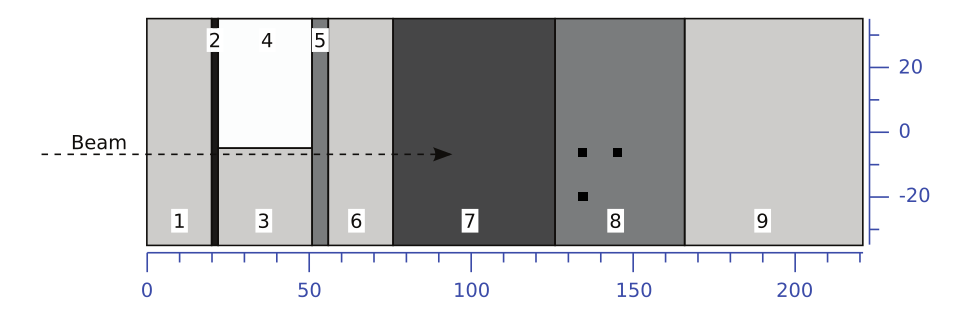
\includegraphics[scale = 0.3]{Parodi/heterofant.png}
    \caption{Fantôme composée en (1) (3) (6) et (9) de Polyethylène, en (2) d'os, en (4) de poumon, en (5) et (8) de muscle et en (7) de PMMA}
    \label{hetero phant}
\end{figure}{}

\subsubsection{Fantôme réaliste}

\subsection{Implémentation de l'information temporelle dans le vpgTLE}


\section{Résultats}

\subsection{\'Etude de la corrélation entre énergie et temps d'émission des gammas}

\subsubsection{Fantôme homogène}
\begin{figure}[h!]
\centering
\subfloat(a){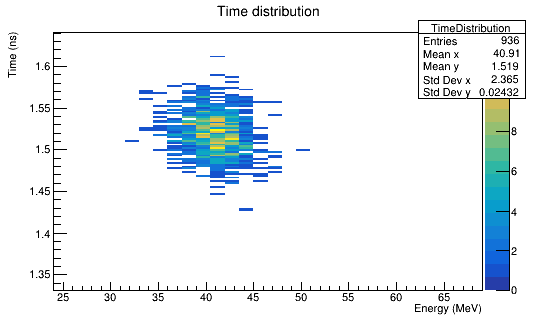
\includegraphics[scale=0.3]{homo/away.png}}
\subfloat(b){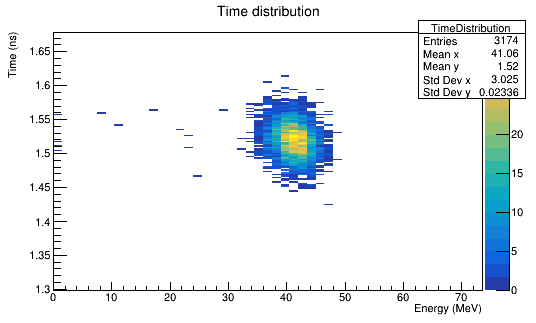
\includegraphics[scale=0.3]{homo/prebragg.png}}\\
\subfloat(c){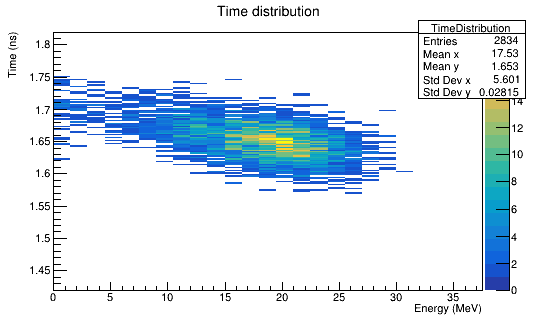
\includegraphics[scale=0.3]{homo/Bragg.png}}
\label{homo prot}
\caption{ Distribution des protons dans (a) un VoI éloigné du faisceau, (b) VoI dans le faisceau avant pic de Bragg et (c) VoI dans le pic de Bragg }

\end{figure}

\begin{figure}[h!]
\centering
\subfloat(a){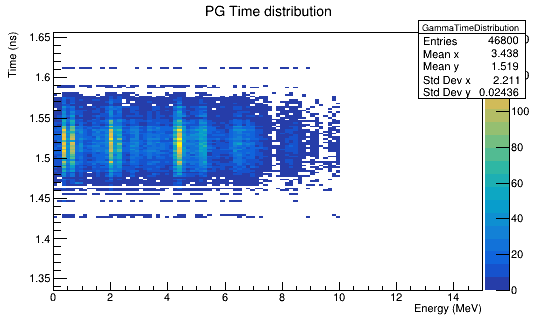
\includegraphics[scale=0.3]{homo/PG/away.png}}
\subfloat(b){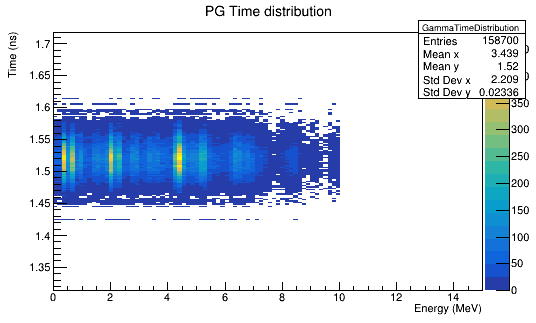
\includegraphics[scale=0.3]{homo/PG/preBragg.png}}\\
\subfloat(c){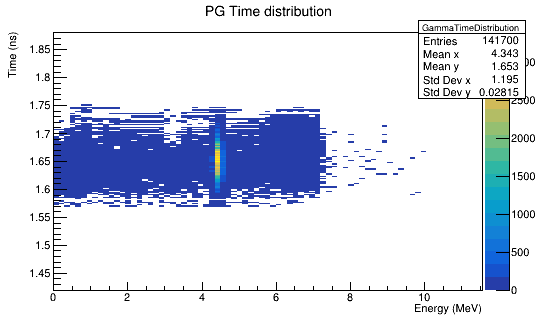
\includegraphics[scale=0.3]{homo/PG/postBragg.png}}
\label{homo pg}
\caption{ Distribution des gamma prompt dans (a) un VoI éloigné du faisceau, (b) VoI dans le faisceau avant pic de Bragg et (c) VoI dans le pic de Bragg }

\end{figure}{}


\subsubsection{Fantôme hétérogène}
\begin{figure}[h!]

\centering
\subfloat(a){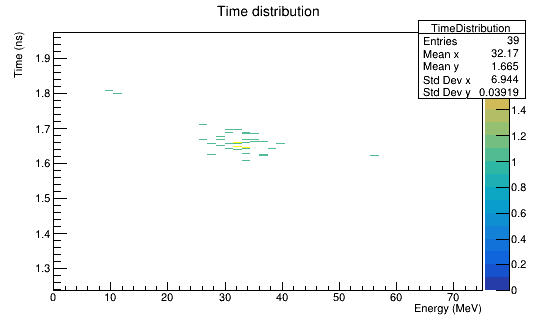
\includegraphics[scale=0.3]{Parodi/away.png}}
\subfloat(b){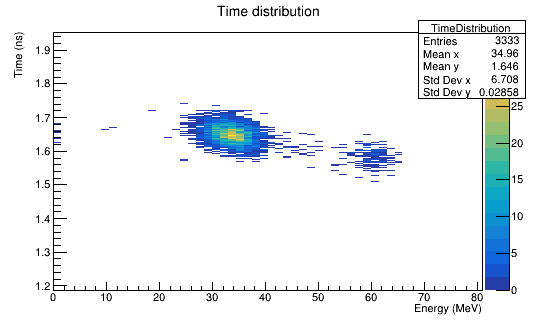
\includegraphics[scale=0.3]{Parodi/preBragg.png}}\\
\subfloat(c){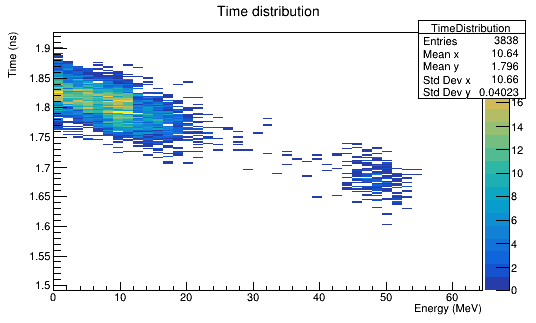
\includegraphics[scale=0.3]{Parodi/Bragg.png}}
\caption{ Distribution de protons dans (a) un VoI éloigné du faisceau, (b) VoI dans le faisceau avant pic de Bragg et (c) VoI dans le pic de Bragg }
\label{hetero prot}
\end{figure}

\begin{figure}[h!]

\centering
\subfloat(a){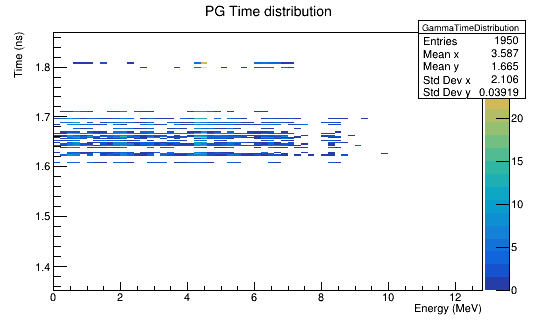
\includegraphics[scale=0.3]{Parodi/PG/away.png}}
\subfloat(b){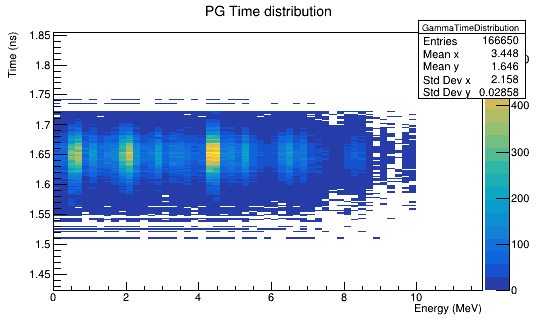
\includegraphics[scale=0.3]{Parodi/PG/preBragg.png}}\\
\subfloat(c){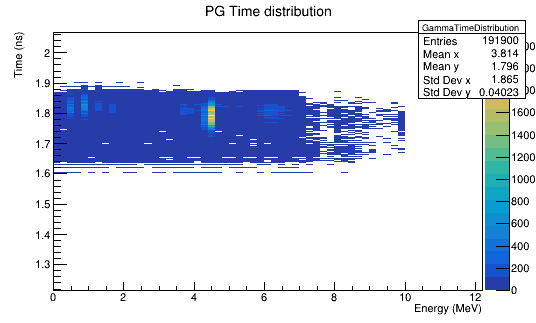
\includegraphics[scale=0.3]{Parodi/PG/Bragg.png}}
    
\caption{ Distribution de PG dans (a) un VoI éloigné du faisceau, (b) VoI dans le faisceau avant pic de Bragg et (c) VoI dans le pic de Bragg }
\label{hetero pg}
\end{figure}


\subsubsection{Fantôme réaliste}

\paragraph{Faisceau monoénergétique}

Fantôme issu d'un plan de traitement ORL représentant un cas réaliste présentant des hétérogénéités. Il est divisé en voxel de $2^{3}~mm^{3}$. 
  
\begin{figure}[h!]
\centering
\subfloat(a){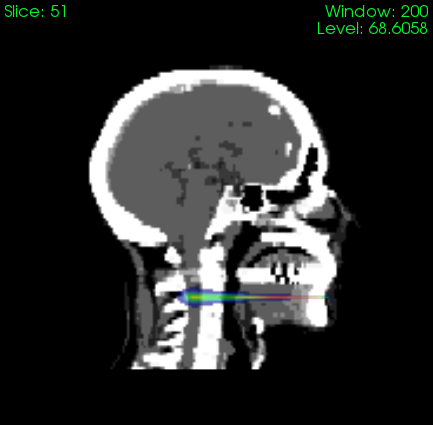
\includegraphics[scale=0.37]{CT/130/profil.png}}
\subfloat(b){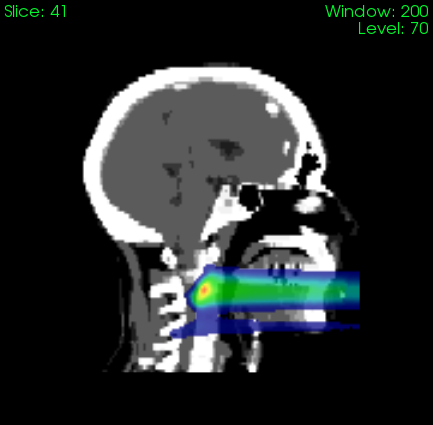
\includegraphics[scale=0.37]{CT/TPS/profil.png}}
\caption{Distribution de la dose dans le fantôme pour (a) le faisceau mono-énergétique de 130~MeV et (b) le faisceau issu du plan de traitement}
\label{profil}
\end{figure}



\paragraph{Faisceau issu d'un plan de traitement}
\begin{figure}[h!]
\centering
\subfloat(a){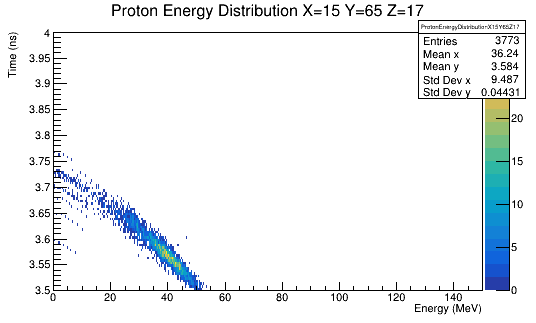
\includegraphics[scale=0.37]{CT/TPS/faisceauprot.png}}
\subfloat(b){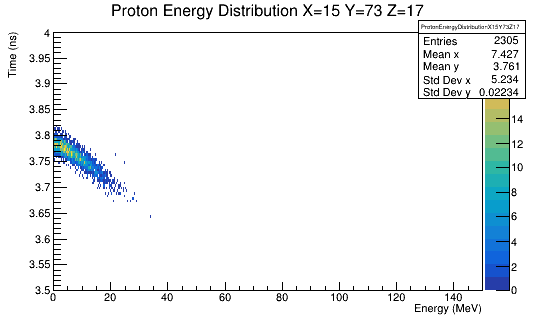
\includegraphics[scale=0.37]{CT/TPS/BraggProt.png}}
\caption{Distribution d'énergie de proton au milieu du faisceau (a) et au pic de Bragg (b)}
\label{tps prot}
\end{figure}

\begin{figure}[h!]
\centering
\subfloat(a){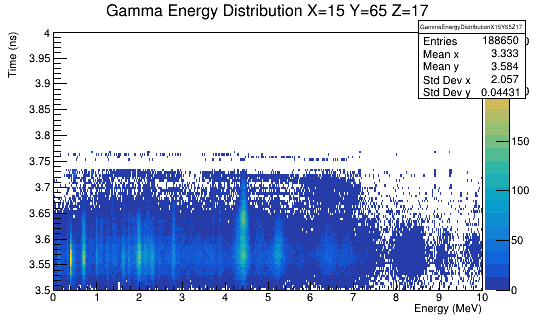
\includegraphics[scale=0.37]{CT/TPS/faisceaugamma.png}}
\subfloat(b){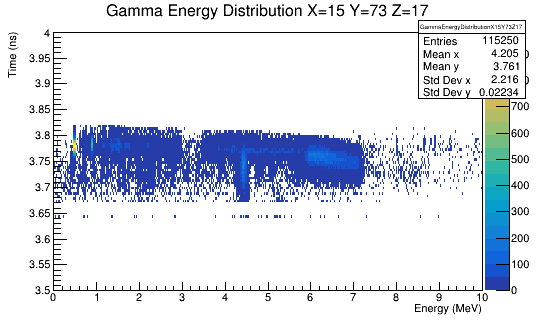
\includegraphics[scale=0.37]{CT/TPS/BraggGamma.png}}
\caption{Distribution d'énergie de gamma prompt au milieu du faisceau (a) et au pic de Bragg (b)}
\label{tps pg}
\end{figure}

\subsection{Implémentation de l'information temporelle dans le vpgTLE}

\section{Discussion}
\subsection{\'Etude de la corrélation entre énergie et temps d'émission des gammas}
Dans les trois cas de cette étude et pour tout les volumes nous trouvons un écart type de l'ordre de la dizaines de picosecondes. Or la résolution temporelle des détecteurs investigué dans le cadre de la collaboration CLaRys est de de 100~ps, dans cette limite nous stockerons donc le temps de vol indépendamment de l'énergie.  

\subsection{Implémentation de l'information temporelle dans le vpgTLE}


\bibliographystyle{apalike}
\bibliography{references}

\newpage

\appendix

\subsubsection{Résultats faisceau mono-énergétique A enlever ??}
\begin{figure}[h!]
\centering
\subfloat(a){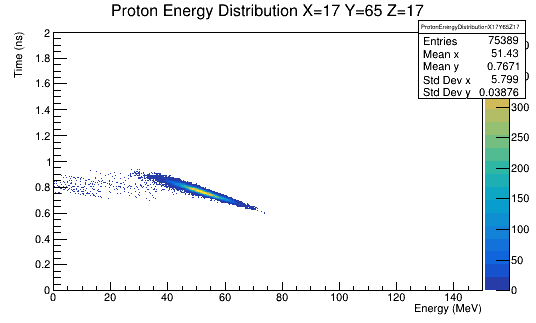
\includegraphics[scale=0.37]{CT/130/FaisceauProt.png}}
\subfloat(b){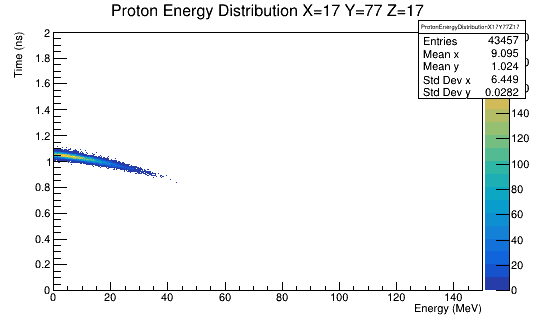
\includegraphics[scale=0.37]{CT/130/BraggProt.png}}
\caption{Distribution d'énergie de proton au milieu du faisceau (a) et au pic de Bragg (b)}
\label{130 prot}
\end{figure}

\begin{figure}[h!]
\centering
\subfloat(a){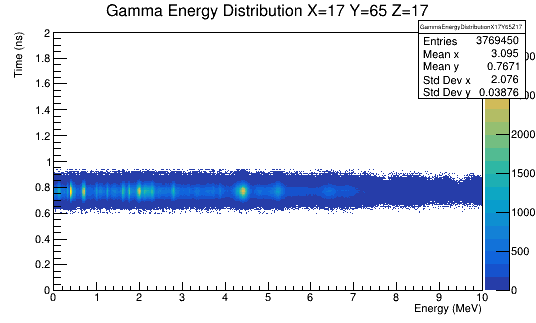
\includegraphics[scale=0.37]{CT/130/FaisceauGamma.png}}
\subfloat(b){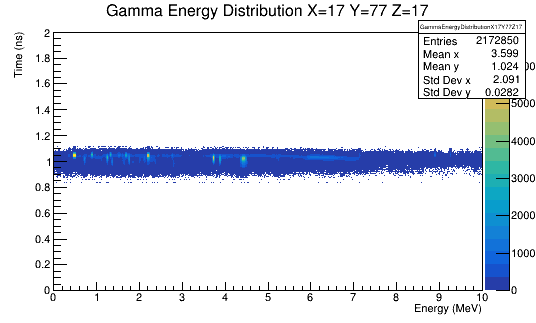
\includegraphics[scale=0.37]{CT/130/BraggGamma.png}}
\caption{Distribution d'énergie de gamma prompt au milieu du faisceau (a) et au pic de Bragg (b)}
\label{130 pg}
\end{figure}
\newpage

\end{document}
